\section{Interference Calculation}

\subsection{Interference Calculation Overview}

Interference calculation is the process of judging whether two sets of geometric models intersect and finding the distance between them. It mainly provides the following two functions:
\begin{itemize}
  \item Collision detection to determine if two models intersect (collision-check function)
  \item A distance calculator that calculates the shortest distance between two models (collision-distance function)
\end{itemize}

In irteus, interference calculations are performed by calling external libraries through other language interfaces. As an external library, calls to PQP and Bullet are implemented, and PQP is used by default. The library to be used can be switched by the select-collision-algorithm function as follows:
{\baselineskip=10pt
\begin{verbatim}
(select-collision-algorithm *collision-algorithm-pqp*) ;; use PQP
(select-collision-algorithm *collision-algorithm-bullet*) ;; use Bullet
\end{verbatim}
}

The features of each external library are described in detail below. See http://gamma.cs.unc.edu/research/collision/ for other interference calculation software packages. (Note that the information may be outdated. For example, Bullet is not listed.)

\input{irtcollision-func}

\subsubsection{Interference Calculation Example Between Object Shape Models}
Below is an example of using collision-check and collision-distance to detect the collision between two cubes, calculate the distance, and draw a line connecting the nearest points. The specifications of the closest point obtained by the collision-distance function when interference occurs are different between PQP and Bullet. For details, see the description of Bullet below:
{\baselineskip=10pt
\begin{verbatim}
;; Make models
(setq *b0* (make-cube 100 100 100))
(setq *b1* (make-cube 100 100 100))

;; Case 1 : no collision
(send *b0* :newcoords (make-coords :pos #f(100 100 -100)
                                   :rpy (list (deg2rad 10) (deg2rad -20) (deg2rad 30))))
(objects (list *b0* *b1*))
(print (collision-check *b0* *b1*)) ;; Check collision
(let ((ret (collision-distance *b0* *b1*))) ;; Check distance and nearest points
  (print (car ret)) ;; distance
  (send (cadr ret) :draw-on :flush nil :size 20 :color #f(1 0 0)) ;; nearest point on *b0*
  (send (caddr ret) :draw-on :flush nil :size 20 :color #f(1 0 0)) ;; nearest point on *b1*
  (send *irtviewer* :viewer :draw-line (cadr ret) (caddr ret))
  (send *irtviewer* :viewer :viewsurface :flush))

;; Case 2 : collision
(send *b0* :newcoords (make-coords :pos #f(50 50 -50)
                                   :rpy (list (deg2rad 10) (deg2rad -20) (deg2rad 30))))
(objects (list *b0* *b1*))
(print (collision-check *b0* *b1*)) ;; Check collision
(let ((ret (collision-distance *b0* *b1*))) ;; Check distance and nearest points
  (print (car ret)) ;; distance
  ;; In case of collision, nearest points are insignificant values.
  (send (cadr ret) :draw-on :flush nil :size 20 :color #f(1 0 0)) ;; nearest point on *b0*
  (send (caddr ret) :draw-on :flush nil :size 20 :color #f(1 0 0)) ;; nearest point on *b1*
  (send *irtviewer* :viewer :draw-line (cadr ret) (caddr ret))
  (send *irtviewer* :viewer :viewsurface :flush))
\end{verbatim}
}

\begin{figure}[htb]
  \begin{center}
    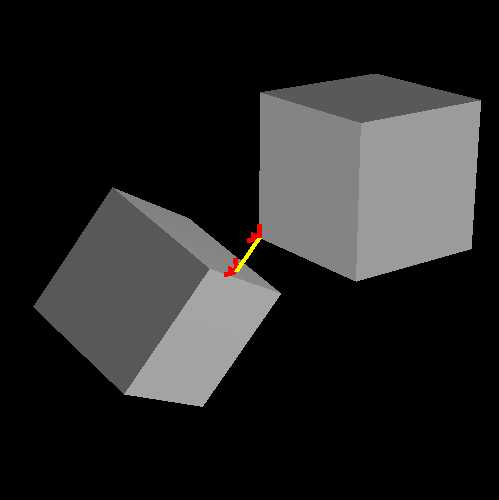
\includegraphics[width=0.50\columnwidth]{fig/collision.jpg}
    \caption{Collision detection}
  \end{center}
\end{figure}

\subsubsection{Robot Motion and Interference Calculation}
When performing a static simulation of the action of grabbing an object with the hand, it is possible to investigate the interference between the links of the hand (fingers) and the target object, and stop the action of grabbing the object when this occurs.

{\baselineskip=10pt
\begin{verbatim}
(load "irteus/demo/sample-arm-model.l")
(setq *sarm* (instance sarmclass :init))
(send *sarm* :reset-pose)
(setq a 42)
(send *sarm* :move-fingers a)
(setq *target* (make-cube 30 30 30))
(send *target* :translate #f(350 200 400))
(objects (list *sarm* *target*))

(send *sarm* :inverse-kinematics *target* :move-target (send *sarm* :end-coords) :debug-view t)
(while (> a 0)
  (if (collision-check-objects
       (list (send *sarm* :joint-fr :child-link)
             (send *sarm* :joint-fl :child-link))
       (list *target*))
      (return))
  (decf a 0.1)
  (send *irtviewer* :draw-objects)
  (send *sarm* :move-fingers a))
(send *sarm* :end-coords :assoc *target*)

(dotimes (i 100)
  (send *sarm* :joint0 :joint-angle 1 :relative t)
  (send *irtviewer* :draw-objects))
(send *sarm* :end-coords :dissoc *target*)
(dotimes (i 100)
  (send *sarm* :joint0 :joint-angle -1 :relative t)
  (send *irtviewer* :draw-objects))
\end{verbatim}
}

Similar functionality is provided by the methods :open-hand and :close-hand in the "irteus/demo/sample-arm-model.l" file.

\subsection{Interference Calculation by PQP}

PQP is an interference calculation library developed by Lin et al.'s group at the University of North Carolina. The usage of the PQP software package is described in irteus/PQP/README.txt, and can be understood by reading irteus/PQP/src/PQP.h.

The files for using PQP with irteus consist of CPQP.C, euspqp.c, and pqp.l.
To determine if two geometric models will collide,
{\baselineskip=10pt
\begin{verbatim}
(defun pqp-collision-check (model1 model2
				       &optional (flag PQP_FIRST_CONTACT) &key (fat 0) (fat2 nil))
  (let ((m1 (get model1 :pqpmodel))  (m2 (get model2 :pqpmodel))
        (r1 (send model1 :worldrot)) (t1 (send model1 :worldpos))
        (r2 (send model2 :worldrot)) (t2 (send model2 :worldpos)))
    (if (null fat2) (setq fat2 fat))
    (if (null m1) (setq m1 (send model1 :make-pqpmodel :fat fat)))
    (if (null m2) (setq m2 (send model2 :make-pqpmodel :fat fat2)))
    (pqpcollide r1 t1 m1 r2 t2 m2 flag)))
\end{verbatim}
}
should be called. 
r1,r1,r2,t1 are the translation vector and rotation matrix of each object, and (get model1 :pqpmodel) refers to the pointer to the PQP geometric model. This pointer is computed in the :make-pqpmodel method as follows.
{\baselineskip=10pt
\begin{verbatim}
(defmethod cascaded-coords
  (:make-pqpmodel
   (&key (fat 0))
   (let ((m (pqpmakemodel))
         vs v1 v2 v3 (id 0))
     (setf (get self :pqpmodel) m)
     (pqpbeginmodel m)
     (dolist (f (send self :faces))
       (dolist (poly (face-to-triangle-aux f))
         (setq vs (send poly :vertices)
               v1 (send self :inverse-transform-vector (first vs))
               v2 (send self :inverse-transform-vector (second vs))
               v3 (send self :inverse-transform-vector (third vs)))
         (when (not (= fat 0))
           (setq v1 (v+ v1 (scale fat (normalize-vector v1)))
                 v2 (v+ v2 (scale fat (normalize-vector v2)))
                 v3 (v+ v3 (scale fat (normalize-vector v3)))))
         (pqpaddtri m v1 v2 v3 id)
         (incf id)))
     (pqpendmodel m)
     m)))
\end{verbatim}
}
Here, (pqpmakemodel) is called first.
In pqpmakemodel, defined in euqpqp.c,

{\baselineskip=10pt
\begin{verbatim}
pointer PQPMAKEMODEL(register context *ctx, int n, register pointer *argv)
{
    int addr = PQP_MakeModel();
    return makeint(addr);
}
\end{verbatim}
}

is invoked, which is the same as in CPQP.C
{\baselineskip=10pt
\begin{verbatim}
PQP\_Model *PQP_MakeModel()
{
    return new PQP_Model();
}
\end{verbatim}
}
PQP\_Model() is defined in PQP.h. After the functions in euslisp are passed to the actual PQP library functions in this way, an instance of the PQP geometric model is created with (pqpbeginmodel m) and the surface information is registered as (pqpaddtri m v1 v2 v3 id) to register the surface information.

\input{pqp-func}

\subsection{Interference Calculation with Bullet}

Bullet is a physics engine, and as part of it, an interference calculation function is provided.
The files for using Bullet with irteus consist of CBULLET.cpp, eusbullet.c, and bullet.l.
The calling order inside the function is the same as PQP.

The differences between PQP and Bullet are as follows.
\begin{itemize}
  \item If you call collision-distance when there is interference, PQP will return 0 as the distance and a meaningless point as the closest point. Bullet, on the other hand, returns the shortest distance (called penetration depth) that should be moved to eliminate interference as the distance. Also, as the closest point, the points at both ends of the shortest distance to eliminate interference are returned.
  \item PQP can handle non-convex mesh models as is, but Bullet internally computes and handles the convex hull of non-convex models.
\end{itemize}

\input{bullet-func}
